
\subsection{Esercizio circuito magnetico}
Si realizza un circuito magnetico come in figura
\begin{figure}[H]
\centering
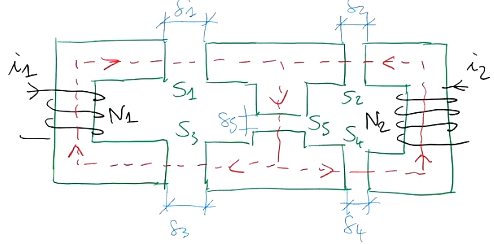
\includegraphics[width = 0.5\linewidth]{esercizio_circuito_magnetico}
\end{figure}

Si vogliono determinare i coefficienti di auto e mutua induzione del circuito, i dati
sono:
$$
\begin{aligned}
&N_1 = 400 \qquad N_2 = 200\\
&\delta_1 = \delta_3 = \SI{2}{\milli\meter}\\
&\delta_2=\delta_4 = \SI{3}{\milli\meter} \\
&\delta_5 = \SI{5}{\milli\meter}\\
&S_1 = S_2 = S_3 = S_4 = S_\delta = \SI{25}{\milli\meter^2}
\end{aligned}
$$
Orientati i flussi si può realizzare l'equivalente circuitale
\begin{figure}[H]
\centering
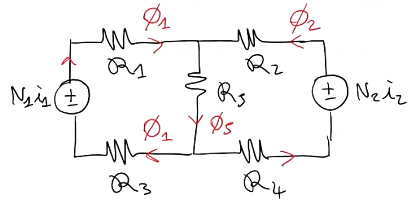
\includegraphics[width = 0.4\linewidth]{esercizio_circuito_magnetico_equivalente_resistivo}
\end{figure}
Si calcolano le riluttanze
$$\begin{aligned}
&\mathcal{R}_1 = \frac{\delta_1}{\mu_0 S} = \mathcal{R}_3 = \frac{\SI{2e-3}{}}{\mu_0\cdot\SI{25e-6}{}} = \SI{6.37e7}{\henry^{-1}}\\
&\mathcal{R}_2 = \frac{\delta_2}{\mu_0S} = \mathcal{R}_4 = \frac{\SI{3e-3}{}}{\mu_0\cdot\SI{25e-6}{}} = \SI{9.55e7}{\henry^{-1}}\\
&\mathcal{R}_5 = \frac{\delta_5}{\mu_0S} = \frac{\SI{5e-3}{}}{\mu_0\cdot\SI{25e-6}{}} = \SI{15.9e7}{\henry^{-1}}\end{aligned}
$$
\newpage
I flussi concatenati da calcolare sono 
$$
\begin{aligned}
&\Phi_1^c = N_1\Phi_1\\
&\Phi_2^c = N_2\Phi_2
\end{aligned}
$$
e quindi i coefficienti di auto e mutua induzione
$$
\begin{aligned}
L_1 &= \left.\frac{\Phi_1^c}{i_1}\right|_{i_2=0} = \frac{N_1\Phi_1'}{i_1}\\
M_{21} &= \left.\frac{\Phi_2^c}{i_1}\right|_{i_2=0} = \frac{N_2\Phi_2'}{i_1}
\end{aligned}
$$
I flussi si calcolano ricavando la riluttanza equivalente ed eseguendo un partitore
di corrente
$$
\begin{aligned}
\Phi_1' &= \frac{N_1i_1}{\mathcal{R}_1+\mathcal{R}_3+\mathcal{R}_5//\left(\mathcal{R}_2+\mathcal{R}_4\right)}\\
\Phi_2' &= -\Phi_1' \frac{\mathcal{R}_5}{\mathcal{R}_5+\mathcal{R}_2+\mathcal{R}_4}
\end{aligned}
$$
quindi
$$
\begin{aligned}
L_1 &= \frac{N_1^2}{\mathcal{R}_1 + \mathcal{R}_3 + \mathcal{R}_5//\left(\mathcal{R}_2+\mathcal{R}_4\right)} = \SI{0.48}{\milli\henry}\\
M_{21} &= -\frac{N_2N_1}{\mathcal{R}_1+\mathcal{R}_3+\mathcal{R}_5//\left(\mathcal{R}_2+\mathcal{R}_4\right)}\cdot\frac{\mathcal{R}_5}{\left(\mathcal{R}_5+\mathcal{R}_2+\mathcal{R}_4\right)} = \SI{-0.17}{\milli\henry}
\end{aligned}
$$
Per calcolare ora l'auto-induttanza $L_2$ è necessario spegnere il primo generatore
ma si vede che il circuito è topologicamente simmetrico, dunque si possono sostituire
i valori delle riluttanze corretti nelle relazioni precedenti.
$$\begin{aligned}
\Phi_2'' &= \frac{N_2i_2}{\mathcal{R}_2+\mathcal{R}_4+\mathcal{R}_5//\left(\mathcal{R}_1+\mathcal{R}_3\right)}\\
\Phi_1'' &= -\Phi_2'' \frac{\mathcal{R}_5}{\mathcal{R}_5 + \mathcal{R}_1+\mathcal{R}_3}
\end{aligned}
$$
$$
\begin{aligned}
L_2 &= \frac{N_2^2}{\mathcal{R}_2 + \mathcal{R}_4 +\mathcal{R}_5//\left(\mathcal{R}_1+\mathcal{R}_3\right)} = \SI{0.15}{\milli\henry}\\
M_{12} &= - \frac{N_1N_2}{\mathcal{R}_2+\mathcal{R}_4+\mathcal{R}_5//\left(\mathcal{R}_1+\mathcal{R}_3\right)}\cdot\frac{\mathcal{R}_5}{\left(\mathcal{R}_5+\mathcal{R}_1+\mathcal{R}_3\right)} = \SI{-0.17}{\milli\henry}
\end{aligned}
$$
$M_{12}=M_{21}$ per la reciprocità.

\newpage
\section{Modelli quasi-stazionari dell'elettromagnetismo}
Si suppone che le sorgenti varino nel tempo ma i tempi caratteristici delle variazioni
siano ``sufficientemente lunghi''.
Si richiamano le equazioni di Maxwell
$$
\begin{aligned}
&\oiint_\Sigma\vec{B}\cdot\hat{n}dS = 0\ \ \forall\ \Sigma \text{ chiusa di } \mathbb{R}^3\\
&\oiint_\Sigma\vec{D}\cdot\hat{n}dS = Q_{\text{lib }\Omega_\Sigma} \\
&\oint_\Gamma \vec{E}\cdot\hat{t} dl = - \iint_{S_\gamma} \frac{\partial\vec{B}}{\partial t}\cdot\hat{n}dS \ \ \forall\ \Gamma \text{ chiusa di } \mathbb{R}^3\\
&\oint_\Gamma \vec{H}\cdot\hat{t}dl = i_\Gamma + \iint_{S_\Gamma} \frac{\partial\vec{D}}{\partial t}\cdot\hat{n} dS\\
&\oiint_\Sigma \vec{J}_\text{lib} \cdot\hat{n}dS = - \iiint_{\Omega_\Sigma} \frac{\partial \rho_\text{lib}}{\partial t}dV\ \ \forall\ \Sigma \text{ chiusa di }\mathbb{R}^3
\end{aligned}
$$
Le ultime tre di queste equazioni contengono delle variazioni nel tempo delle grandezze, queste
grandezze sono legate tra loro ma se si suppone di poterle far variare
in maniera indipendente istante per istante. 

Si sviluppano dunque modelli differenti, il primo
se si suppone che resti costante il vettore spostamento $\vec{D}$, prende il nome
di ``Magneto-Quasi-Stazionario'' (MQS) in cui i campi magnetici si determinano a partire dalla
conoscenza delle distribuzioni di corrente e i campi elettrici si ricavano a posteriori.

Il secondo modello che prende il nome di ``Elettro-Quasi-Stazionario'' (EQS) in cui si 
trascura la variazione del campo di induzione magnetica e vale solitamente per i 
dielettrici.

Un terzo modello che generalizza la conduzione stazionaria prende il nome di
``rilassamento della carica'' sempre trascurando la variazione del campo di induzione
magnetica $\vec{B}$, equivale al modello EQS in presenza di conduttori.

Riassumendo
\begin{enumerate}
\item MQS $\rightarrow \frac{\partial\vec{D}}{\partial t},\ \frac{\partial \rho_\text{lib}}{\partial t} \simeq 0$
\item EQS $\rightarrow\frac{\partial\vec{B}}{\partial t} \simeq 0 $ (dielettrici)
\item Rilassamento della carica $\frac{\partial\vec{B}}{\partial t} \simeq 0$ (conduttori)
\end{enumerate}

Si analizza il modello del rilassamento della carica, in forma locale. Si suppone
di avere un certo dominio $\Omega$ che si comporta sia da conduttore che da dielettrico,
caratterizzato dunque da una conducibilità $\gamma$ e una permittività dielettrica
$\varepsilon$ costanti.

Le equazioni di Maxwell in forma locale diventano:
$$
\begin{aligned}
&\text{Nei punti regolari}\\
&\nabla\cdot\vec{D} = \rho_\text{lib} \\
&\nabla\times\vec{E} = 0\\
&\nabla\cdot\vec{J}_\text{lib} = -\frac{\partial \rho_\text{lib}}{\partial t}
\end{aligned}\qquad 
\begin{aligned}
&\text{Sulle superfici di discontinuità e.g. }\partial \Omega\\
&\hat{n}\cdot\left(\vec{D}_2-\vec{D}_1\right) = \sigma_\text{lib}\\
&\hat{n}\times\left(\vec{E}_2-\vec{E}_1\right) = 0\\
&\hat{n}\cdot\left(\vec{J}_2-\vec{J}_1\right) = -\frac{\partial\sigma_\text{lib}}{\partial t}
\end{aligned}
$$
A queste si aggiungono le relazioni costitutive
$$
\begin{aligned}
&\vec{D} = \varepsilon\vec{E}\\
&\vec{J}_\text{lib} = \gamma \vec{E}
\end{aligned}
$$
Sostituendo nelle equazioni di Maxwell
$$
\vec{D} = \varepsilon\frac{\vec{J}_\text{lib}}{\gamma} \Rightarrow \nabla\cdot\left(\frac{\varepsilon}{\gamma}\vec{J}_\text{lib}\right) = \rho_\text{lib}=
\frac{\varepsilon}{\gamma}\nabla\cdot\vec{J}_\text{lib} = \frac{\varepsilon}{\gamma}\left(-\frac{\partial \rho_\text{lib}}{\partial t}\right)
$$

questo implica che 
$$
\tau_e \frac{\partial\rho_\text{lib}}{\partial t} + \rho_\text{lib} = 0
$$
con $\tau_e = \frac{\varepsilon}{\gamma}$ che rappresenta il tempo di rilassamento della
carica libera in un conduttore omogeneo.

La precedente è un'equazione differenziale a derivate parziali dato che $\rho_\text{lib}$
è funzione del tempo ma anche del punto $p'$, la sua soluzione generale è
$$
\rho_\text{lib}(p',t) = \rho_\text{lib}(p',t=0)e^{-\frac{t}{\tau_e}}
$$
dove il termine per $t=0$ è la distribuzione di carica iniziale.

L'equazione vale indipendentemente da ciò che accade nel dominio $\Omega$ ossia in un 
conduttore omogeneo la carica libera si distribuisce sulla superficie di frontiera $\partial\Omega$ in un tempo pari a $(4\div 5)\ \tau_e$.
Sul conduttore non sono presenti dunque distribuzioni di cariche libere di volume ma 
solo distribuzioni di cariche superficiali.

Se le variazioni delle sorgenti sono molto più lente di $\tau_e$ è possibile applicare
il modello di corrente quasi-stazionaria.
\newpage
\subparagraph{Esempio numerico}
$$
\varepsilon = \varepsilon_r\varepsilon_0,\qquad \varepsilon_0 = \SI{8.85e-12}{\farad\per\meter}
$$
$$
\gamma = 
\begin{cases}
\gamma_{Cu} &\simeq \SI{e7}{\siemens\per\meter}\\
\gamma_{H_2O} &\simeq \SI{e-4}{\siemens\per\meter}
\end{cases}
$$
\begin{table}[H]\centering
\begin{tabular}{|c|c|c|c|}
 \hline Materiale & $\gamma[\si{\siemens\per\meter}]$ & $\varepsilon_r$ & $\tau_e[\si{\second}]$ \\
 \hline  &                                          &               &               \\
 $Cu$        & $\SI{5.8e7}{}$                    &   1           &   $\SI{1.5e-19}{}$ \\ 
 $H_2O$           & $\SI{2e-4}{} $                   &       81         & $\SI{3.6e-6}{}$ \\  
 Mica               & $\SI{e-11}{}\div\SI{e-15}{}$       &  5.8        &   $\SI{5.1}{}\left(1\div\SI{e4}{}\right)$ \\ \hline
\end{tabular}
\end{table}

Nel caso in cui il materiale non fosse omogeneo, l'analisi risulterebbe troppo complessa per gli
obbiettivi del corso e non verrà trattata. Si suppone invece che i materiali siano sempre almeno 
omogenei a tratti.

\paragraph{Modello Quasi-Stazionario-Magnetico MQS}
$\frac{\partial\vec{D}}{\partial t} \to 0$, $\frac{\partial\rho_\text{lib}}{\partial t}\to 0$
Si suppone che ci sia una distribuzione di correnti assegnate in una certa regione causa
di un campo di induzione magnetica $\vec{B}$ nello spazio per la legge di Biot-Savart.

Si vuole estendere questo fenomeno a correnti variabili nel tempo in maniera quasi 
stazionaria affinché non ci siano correnti di spostamento.

Sia presente un circuito quasi filiforme attraversato da una corrente $i$, si ipotizza 
inoltre che sia presente nello spazio una regione conduttiva $\Omega_c$ ipotizzando
che ci sia una permeabilità magnetica assegnata e che sia in prima approssimazione un
conduttore perfetto. Il materiale è dunque lineare dal punto di vista magnetico
oppure se ferromagnetico, il punto di lavoro è ancora nella regione lineare di un 
materiale SOFT.

Le equazioni del modello MQS in forma locale sono
$$
\begin{aligned}
&\nabla\cdot\vec{B} = 0\qquad\qquad\ \text{in }\Omega\\
&\nabla\times\vec{H} = \vec{J}_\text{lib} \qquad\ \  \text{in } \Omega_\infty-\Omega_c\\
&\nabla\times\vec{E} = -\frac{\partial\vec{B}}{\partial t} \qquad \text{in } \Omega_\infty-\Omega_c
\end{aligned}
$$
Nel conduttore perfetto il campo elettrico è nullo anche in presenza di correnti 
libere
$$
\vec{E}=0,\ \vec{J}_\text{lib} \neq 0
$$
e quindi sarà nullo anche il rotore del campo, di conseguenza
$$
\nabla\times\vec{E} = -\frac{\partial\vec{B}}{\partial t} \Rightarrow \frac{\partial\vec{B}}{\partial t} = 0
$$
Quindi il campo $\vec{B}$ resta costante nel conduttore e nell'ipotesi di sistema a riposo 
iniziale, questo resta nullo.

In un conduttore perfetto non può penetrare un campo di induzione magnetica e in 
particolare sulla superficie
$$
\hat{n}\cdot\vec{B} = 0
$$
un conduttore ideale ha quindi al suo interno un campo elettrico nullo e un campo
di induzione magnetica nullo.

Nello spazio non occupato dal conduttore invece $\Omega_\infty-\Omega_c$ si suppone
che la variazione delle correnti sia più lenta di $\tau_e$ quindi la carica di volume 
è nulla istante per istante $(\rho = 0 )$ e quindi anche la divergenza del campo $\nabla\cdot\vec{E} = 0$
è nulla nello spazio.

Le equazioni che descrivono il campo elettrico indotto
$$
\begin{aligned}
&\nabla\cdot\vec{E} = 0\\
&\nabla\times\vec{E} = -\frac{\partial\vec{B}}{\partial t}\\
&\hat{n}\cdot\left(\vec{E}_2-\vec{E}_1\right) = \frac{\sigma}{\varepsilon_0} \qquad \text{su }\partial(\Omega_\infty-\Omega_c) \\
& \hat{n}\times\left(\vec{E}_2-\vec{E}_1\right) = 0
\end{aligned}
$$
mediante la legge di Biot-Savart si scompone il campo $\vec{E}$ in due parti, quella prodotta
dal campo $\vec{B}$ e quella prodotta dalle cariche $\sigma$

Dunque il campo $\vec{E}_B$ prodotto dall'induzione magnetica si descrive come
$$
\begin{aligned}
&\nabla\cdot\vec{E}=0\\
&\nabla\times\vec{E} = -\frac{\partial \vec{B}}{\partial t}\\
&\hat{n}\cdot\left( \vec{E}_2-\vec{E}_1  \right) = 0
\end{aligned}
$$
ma questo modello è identico a quello del campo magnetostatico prodotto da una
distribuzione di correnti assegnata
$$\begin{aligned}
&\nabla\cdot\vec{B}=0\\
&\nabla\times\vec{B} = -\frac{\partial \vec{B}}{\partial t}\\
&\hat{n}\cdot\left( \vec{B}_2-\vec{B}_1  \right) = 0\\
&\hat{n}\times\left(\vec{B}_2-\vec{B}_1\right) = 0 \quad \text{senza correnti superficiali}
\end{aligned}
$$
Il campo $\vec{E}_B$ si ottiene dunque mediante la legge di Biot-Savart
$$
\vec{B} = \frac{\mu_0}{4\pi} \iiint_{\Omega_\infty - \Omega_C} \vec{J}\times
\frac{\vec{r}_p-\vec{r}_{p'}}{|\vec{r}_p-\vec{r}_{p'}|^3} dV
$$
che confrontata con l'integrale del rotore di $\vec{B}$
$$
\vec{E}_B = -\frac{1}{4 \pi} \iiint_{\Omega_\infty - \Omega_C} \frac{\partial\vec{B}}{\partial t} \times \frac{\vec{r}_p - \vec{r}_{p'}}{\left|\vec{r}_p - \vec{r}_{p'}\right|^3} dV
$$
permette di calcolare il campo $\vec{E}_B$ elettrico indotto dalla variazione di campo
di induzione magnetica nel tempo.

Per calcolare l'altro termine $\vec{E}_\sigma$ si avranno equazioni differenti come:
$$
\begin{aligned}
&\nabla\cdot\vec{E}=0\\
&\nabla\times\vec{E} = 0\qquad\qquad\quad\ \ \text{ su }\Omega_\infty-\Omega_C\\
&\hat{n}\cdot\left(\vec{E}_2-\vec{E}_1\right) = \frac{\sigma}{\varepsilon_0}\qquad \text{su }\partial\left(\Omega_\infty-\Omega_c\right)
\end{aligned}
$$
se il campo $\vec{E}$ è conservativo, si può esprimere il campo come gradiente di una funzione potenziale e risolvere le equazioni al contorno
$$
\vec{E}=-\nabla\varphi \Rightarrow \begin{cases}
\nabla^2 \varphi = 0\\
-\frac{\partial \varphi_2}{\partial n} + \frac{\partial \varphi_1}{\partial n} = \frac{\sigma}{\varepsilon_0} \text{ su } \partial\left(\Omega_\infty - \Omega_C\right)
\end{cases}
$$

Il campo totale dunque
$$
\vec{E} = \vec{E}_B + \vec{E}_\sigma
$$
rispetterà la continuità delle componenti tangenziali su $\partial\left(\Omega_\infty-\Omega_C\right)$
$$
\hat{n}\times\left(\vec{E}_{B_2} - \vec{E}_{B_1}\right) = -\hat{n}\times\left(\vec{E}_{\sigma_2} - \vec{E}_{\sigma_1}\right)
$$

In alternativa introducendo il potenziale vettore $\vec{A}:\ \vec{B}=\nabla\times\vec{A}$
$$
\nabla\times\vec{E} = -\frac{\partial\vec{B}}{\partial t} = \nabla\times\vec{E} = -\nabla
\times\left(\frac{\partial\vec{A}}{\partial t}\right) \Rightarrow \nabla\times\left(
\vec{E}+\frac{\partial\vec{A}}{\partial t}\right) = 0
$$
se la regione è a connessione superficiale semplice, se 
$$
\vec{E} + \frac{\partial \vec{A}}{\partial t} = -\nabla\varphi \Rightarrow \vec{E} = 
-\frac{\partial \vec{A}}{\partial t} - \nabla\varphi
$$


Queste equazioni sono fondamentali per capire le caratteristiche di schermatura di un 
conduttore da un campo magnetico variabile.

\newpage
\subsection{Diffusione del campo magnetico attraverso conduttori sottili}
Si considera una sorta di cilindro cavo con sezione non circolare ma di forma qualsiasi
attraversato da una corrente $\vec{J}$ che corre lungo la superficie laterale, costante
lungo $z$.
$$
\vec{J} = J_x \left(x,y,t\right)\vec{e}_x + J_y\left(x,y,t\right)\vec{e}_y
$$
\begin{figure}[H]
\centering
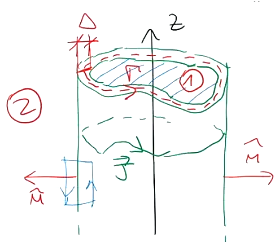
\includegraphics[width = 0.3\linewidth]{schermo_magnetico_cilindrico}
\end{figure}
Si astrae la corrente superficiale
$$
\Delta\to 0,\ J\to \infty:\ J\cdot\Delta = J_S
$$
La legge di Ampére-Maxwell afferma in questo caso
$$
\hat{n}\times\left(\vec{H}_2-\vec{H}_1\right) = \vec{J}_S
$$
ma siccome il versore $\hat{n}$ è ortogonale all'asse $\vec{e}_z$
allora il campo $\vec{H}$ sarà diretto lungo $z$
$$
\vec{H} = H_z\left(x,y,t\right)\vec{e}_z
$$
quindi
$$
H_{z_1} - H_{z_2} = J_S
$$

$H_{z_1}$ e $J_S$ sono incognite da determinare.
Si applica la legge di Faraday-Neumann ad una linea $\Gamma$ che giace nel cilindro
in un piano $x,y$
$$
\oint_\Gamma \vec{E}\cdot\hat{t}dl = -\frac{d}{dt} \iint_{S_\Gamma} \vec{B}\cdot\hat{n}dS
$$
ma nel conduttore $\vec{J} = \gamma\vec{E}$ che sostituita nell'integrale
$$
\oint_\Gamma \frac{\vec{J}}{\gamma}\cdot\hat{t}dl = -\frac{d}{dt} \Phi_\Gamma
$$
Ricordando che lo spessore del foglio è sottile si ha che $\vec{J}\Delta = \vec{J}_S \Rightarrow \vec{J} = \frac{\vec{J}_S}{\Delta}$

$$
\oint_\Gamma \frac{\vec{J}_s}{\Delta\gamma} \cdot\hat{t}dl = -\frac{d}{dt} \Phi_\Gamma
$$

Se $\vec{J}$ è solenoidale (come assunto nel modello MQS) la corrente $\vec{J}_S$ non 
dipende dalla coordinata azimutale $\varphi$, può quindi essere esclusa dall'integrale.
$$
J_S\oint_\Gamma\frac{dl}{\Delta_l\gamma_l} = -\frac{d}{dt}\Phi_\Gamma \Rightarrow
\begin{aligned}
&\Delta_l = \Delta\\
&\gamma_l = \gamma
\end{aligned}
\Rightarrow \frac{J_S L}{\Delta\gamma} = -\frac{d}{dt}\Phi_\Gamma
$$
Se si assume il cilindro omogeneo e $L$ è il perimetro della sua sezione.

Nel caso particolare in cui la sezione del cilindro sia circolare di raggio $a$, la precedente diventa
$$
\frac{J_s 2\pi a}{\Delta\gamma} = -\frac{d}{dt}\left(\mu_0\pi a^2 H_{z_1}\right)
$$
Ricordando la discontinuità della componente tangenziale si ottiene
$$
\frac{H_{z_1} - H_{z_2}}{\Delta\gamma}\cdot 2\cancel{\pi} \cancel{a} = -\frac{d}{dt} \left(\mu_0 \cancel{\pi}a^{\cancel{2}}H_{z_1}\right) \Rightarrow \frac{2H_{z_1}}{\Delta\gamma} - \frac{2H_{z_2}}{\Delta\gamma} = -\mu_0 a \frac{d}{dt}H_{z_1}
$$
Si può riscrivere come
$$
\mu_0\frac{a\Delta\gamma}{2}\frac{dH_{z_1}}{dt} + H_{z_1} = H_{z_2}
$$
dove $\tau_m =  \mu_0\frac{a\Delta\gamma}{2}$ è la costante di tempo della diffusione 
del campo magnetico.

Conoscendo il campo nella regione (2) e risolvendo l'equazione differenziale si ottiene 
l'equazione nel tempo del campo magnetico all'interno del cilindro
$$
\begin{aligned}
& H_{z_2}(t) = H_0u(t)\\
& H_{z_1}(t) = H_0\left(1-e^{-\frac{t}{\tau_m}}\right)
\end{aligned}
$$
Ciò significa che per un tempo $t\ll \tau_m$ l'interno del cilindro è effettivamente 
schermato dal campo esterno, mentre a regime o per un tempo $t > (4\div5)\ \tau_m$ il campo
interno tende ad essere uguale a quello esterno.

La corrente superficiale 
$$
J_S = H_{z_1} - H_{z_2} \stackrel{t>0}{=} H_{z_1} - H_0 = -H_0 e^{-\frac{t}{\tau_m}}
$$
ha un andamento simile al campo $\vec{H}$ ma ha un valore iniziale negativo e tende a zero.
\begin{figure}[H]
\centering
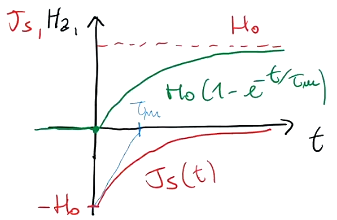
\includegraphics[width = 0.3\linewidth]{campo_e_corrente_schermo_magnetico}
\end{figure}

Essendoci un campo magnetico variabile si può determinare il campo elettrico $\vec{E}$ 
indotto, applicando la legge di Faraday-Neumann ad una linea piana $\Gamma$ di raggio $r$
$$
\oint_\Gamma \vec{E}\cdot\hat{t} dl = -\frac{d}{dt} \iint_{S_\Gamma} \vec{B}\cdot\hat{n}dS
$$
con $\vec{B} = \mu_0 \vec{H}$ e $B_z = \mu_0 H_z$.

Svolgendo gli integrali
$$
\begin{aligned}
&r< a \\
& 2 \cancel{\pi} \cancel{r} E_\varphi = -\frac{d}{dt} \left(\mu_0 H_{z_1}\cancel{\pi} r^{\cancel{2}}\right) \Rightarrow E_\varphi = -\frac{\mu_0}{2}r \frac{dH_{z_1}}{dt}\\
& r >  a \\
& 2\pi r E_\varphi = -\frac{d}{dt} \left(\mu_0 H_{z_1} \pi a^2\right) - \frac{d}{dt} \left(\mu_0 H_{z_2} \pi \left(r^2 - a^2\right)\right)
\end{aligned}
$$

